\documentclass[aspectratio=169]{beamer}

\usepackage{mystyle}

%Concepts
\newcommand{\iot}{IoT\xspace}
\newcommand{\iomt}{IoMT\xspace}
\newcommand{\software}{software\xspace}
\newcommand{\Software}{Software\xspace}
\newcommand{\middleware}{middleware\xspace}
\newcommand{\Middleware}{Middleware\xspace}
\newcommand{\smartobj}{\textit{smart object}\xspace}
\newcommand{\Smartobj}{\textit{Smart object}\xspace}
\newcommand{\smartobjs}{\textit{smart objects}\xspace}
\newcommand{\Smartobjs}{\textit{Smart objects}\xspace}
\newcommand{\broadcast}{\textit{broadcast}\xspace}
\newcommand{\gateway}{gateway\xspace}
\newcommand{\Gateway}{Gateway\xspace}
\newcommand{\gateways}{gateways\xspace}
\newcommand{\Gateways}{Gateways\xspace}
\newcommand{\smartphone}{smart\-phone\xspace}
\newcommand{\Smartphone}{Smart\-phone\xspace}
\newcommand{\smartphones}{smart\-phones\xspace}
\newcommand{\Smartphones}{Smart\-phones\xspace}
\newcommand{\timestamp}{\textit{timestamp}\xspace}
\newcommand{\timestamps}{\textit{timestamps}\xspace}
\newcommand{\framework}{framework\xspace}
\newcommand{\dataset}{\textit{dataset}\xspace}
\newcommand{\Dataset}{\textit{Dataset}\xspace}
\newcommand{\broker}{\textit{broker}\xspace}
\newcommand{\Broker}{\textit{Broker}\xspace}
\newcommand{\brokers}{\textit{brokers}\xspace}
\newcommand{\Brokers}{\textit{Brokers}\xspace}
\newcommand{\ubroker}{\textit{microbroker}\xspace}
\newcommand{\api}{API\xspace}
\newcommand{\pub}{\textit{publisher}\xspace}
\newcommand{\pubs}{\textit{publishers}\xspace}
\newcommand{\sub}{\textit{subscriber}\xspace}
\newcommand{\subs}{\textit{subscribers}\xspace}
\newcommand{\pubsub}{\textit{publisher/subscriber}\xspace}
\newcommand{\listener}{\textit{listener}\xspace}

%Technologies
\newcommand{\rfid}{RFID\xspace}
\newcommand{\ble}{BLE\xspace}
\newcommand{\beacon}{\textit{beacon}\xspace}
\newcommand{\Beacon}{\textit{Beacon}\xspace}
\newcommand{\beacons}{\textit{beacons}\xspace}
\newcommand{\Beacons}{\textit{Beacons}\xspace}
\newcommand{\bluetooth}{\textit{bluetooth}\xspace}
\newcommand{\Bluetooth}{\textit{Bluetooth}\xspace}
\newcommand{\BluetoothLowEnergy}{\textit{Bluetooth Low Energy}\xspace}
\newcommand{\mqtt}{MQTT\xspace}

%Proper noun
\newcommand{\android}{Android\xspace}
\newcommand{\mhub}{M-Hub\xspace}
\newcommand{\cddl}{CDDL\xspace}
\newcommand{\mhubcddl}{M-Hub/CDDL\xspace}
\newcommand{\stwopa}{S2PA\xspace}
\newcommand{\qocevaluator}{\texttt{QoCEvaluator}\xspace}
\newcommand{\eventbus}{EventBus\xspace}
\newcommand{\stwopaservice}{\texttt{S2PAService}\xspace}
\newcommand{\faketechnology}{\texttt{FakeTechnology}\xspace}
\newcommand{\techinterface}{\texttt{Technology}\xspace}
\newcommand{\techlistener}{\texttt{TechnologyListener}\xspace}
\newcommand{\sensordata}{\texttt{SensorData}\xspace}
\newcommand{\msg}{\texttt{Message}\xspace}
\newcommand{\objfoundmsg}{\texttt{ObjectFoundMessage}\xspace}
\newcommand{\objconnectedmsg}{\texttt{ObjectConnectedMessage}\xspace}
\newcommand{\objdisconnectedmsg}{\texttt{ObjectDisconnectedMessage}\xspace}
\newcommand{\sensordatamsg}{\texttt{SensorDataMessage}\xspace}

%Misc
\newcommand{\autoriapropria}{Produzido pelo autor\xspace}

%General
\title{Descoberta e Desconexão de Objetos Inteligentes (\textit{Smart Objects}) em Ambientes Oportunísticos de IoMT}
\author{Alysson Cirilo Silva}
\date{2019}
\institute[LSDi-UFMA]{Laboratório de Sistemas Distribuídos Inteligentes (LSDi)\\Universidade Federal do Maranhão (UFMA)\\\url{http://www.lsdi.ufma.br}}




\begin{document}

\frame{\titlepage}

\begin{frame}
	\frametitle{Sumário}
	\tableofcontents
\end{frame}


\section{Introdução}


\begin{frame}
	\frametitle{\iot}
	\begin{itemize}
		\item paradigma de comunicação onde os objetos do dia a dia são equipados com protocolos e equipamentos que permitem que se comuniquem com outros objetos e seus usuários \cite{atzori:iera:morabito:2010};

		\item Os objetos em um cenário de \iot são denominados \smartobjs.
	\end{itemize}
\end{frame}

\begin{frame}
	\frametitle{\Middleware}
	Camada ou conjunto de camadas de \software entre os níveis tecnológicos e de aplicação.
	Possui característica de esconder detalhes de diferentes tecnologias de forma a facilitar o desenvolvimento de aplicações, fazendo com que o desenvolvedor se concentre nos problemas pertinentes ao seu domínio.
	Se tornando fundamental para cenários de \iot \cite{atzori:iera:morabito:2010}.
\end{frame}

\begin{frame}
	\frametitle{\iomt}
	\begin{itemize}
		\item extensão da \iot;
			
		\item \smartobjs e \textbf{\gateways} são livres para se locomover;

		\item maior dinamicidade de iterações.
	\end{itemize}
\end{frame}

\begin{frame}
	\frametitle{Diferenças importantes entre \iot e \iomt \cite{nahrstedt:et-al:2016}}
	\begin{itemize}

		\item {contexto};

		\item {acesso à Internet e conectividade};

		\item {disponibilidade de energia};

		\item {segurança e privacidade}.

	\end{itemize}
\end{frame}

\begin{frame}
	\frametitle{\mhubcddl}
	\begin{itemize}
		\item \middleware \iomt desenvolvido na plataforma \android para aquisição, processamento e distribuição de dados de contexto;
			
		\item amplo suporte para criação de aplicações de \iot cientes de contexto que possuam requisitos de qualidade de contexto \cite{gomes:et-al:2017};

		\item desenvolvido em parceria da UFMA com a PUC-Rio.
	\end{itemize}
\end{frame}

\begin{frame}
	\frametitle{Caracterização do problema}
	Dado a dinamicidade da \iomt, onde os \smartobjs e \gateways interagem de forma oportunística, torna-se claro a necessidade da existência de um mecanismo de notificação de eventos de descoberta, conexão e desconexão de \smartobjs com os \smartphones.
\end{frame}

\begin{frame}
	\frametitle{Objetivos}
	\begin{itemize}
		\item implementar o mecanismo de notificação no \middleware \mhubcddl;

		\item realizar análises de performance e percentual de perdas na solução proposta.
	\end{itemize}
		
	
\end{frame}


\section{Fundamentação teórica}


\begin{frame}
	\frametitle{\mqtt}
	\begin{itemize}
		\item protocolo baseado em mensagens seguindo o modelo \pubsub;

		\item baseado em tópicos que são gerenciados por \brokers;

		\item projetado para o uso em redes não confiáveis;

		\item consistem em um servidor \broker e dois tipos de clientes: \pubs e \subs;
			
		\item protocolo padrão utilizado pelo \cddl para realizar troca de mensagens entre diferentes componentes.
	\end{itemize}
\end{frame}

\begin{frame}
	\frametitle{\Broker}
	\begin{itemize}
		\item intermedeia as mensagens enviadas pelos \pubs e recebidas pelos \subs;

		\item organiza as mensagens por meio de tópicos:
			\begin{itemize}
				\item funcionam como uma hieraquía de diretórios onde as mensagens são entregues.
			\end{itemize}

		\item os \pubs publicam mensagens em um tópico de um \broker;

		\item o \broker se encarrega de entregar as mensagens para os \subs que registraram interesse;
	\end{itemize}
\end{frame}

\begin{frame}
	\frametitle{Processo de entrega de mensagens \mqtt}
	\begin{figure}
		\centering
		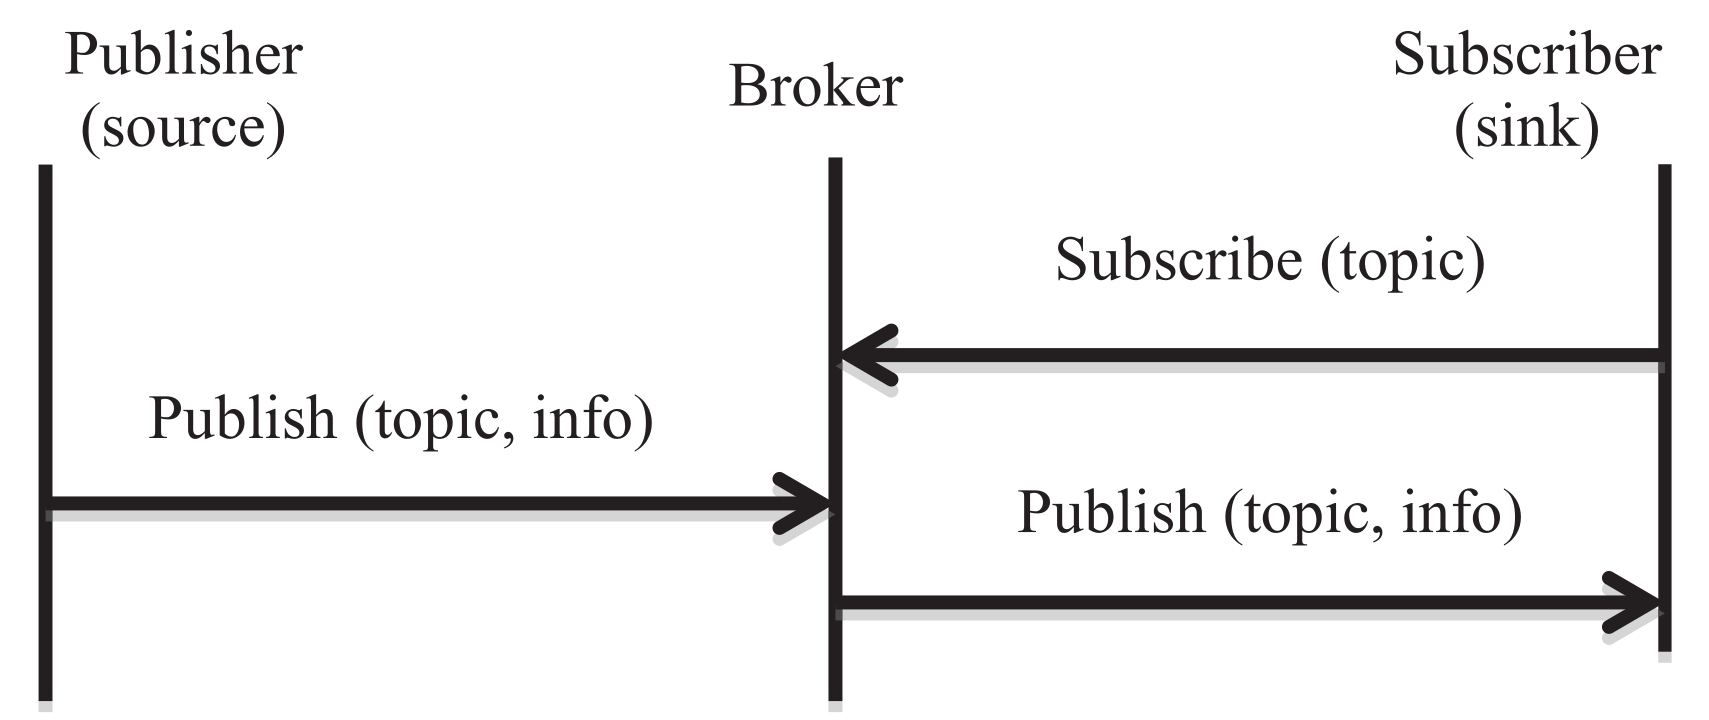
\includegraphics[width=.70\linewidth]{img/mqtt-sequence.png}
		\caption{Fonte:\cite{al-fuqaha:et-al:2015}}
	\end{figure}
\end{frame}

\begin{frame}
	\frametitle{Tópicos \mqtt}
	Ao publicar um dado no \broker \mqtt, o produtor de dados especifíca um tópico onde este dado será publicado.
	O tópico pode possuir um ou mais níveis de hieraquía, com cada nível sendo separado por uma barra, como:
	\begin{itemize}
		\item \texttt{thailand/humidity};
		\item \texttt{thailand/bangkok/traffic}.
	\end{itemize}
\end{frame}

\begin{frame}
	\frametitle{Tópicos \mqtt}
	Também existe a conveniência da utilização de caracteres coringas para a assinatura de tópicos.
	Os caracteres disponíveis são:
	\begin{itemize}
		\item ``\texttt{+}'': Substitui um nível na hierarquía;
		\item ``\texttt{\#}'': Substitui todos os níveis subsequentes na hierarquía;
	\end{itemize}
	
	Como exemplo: o tópico ``\texttt{thailand/+/traffic}'' pode ser utilizado para receber os dados de tráfego de qualquer cidade da Tailândia~\cite{hunkeler:truong:stanford-clark:2008}.
\end{frame}

\begin{frame}
	\frametitle{Tópicos \mqtt}
	Dado o seguinte tópico \texttt{a/b/c/d}, as seguintes assinaturas irão receber os dados publicados nele \cite{light:mosquitto}:
	\begin{itemize}
		\item \texttt{a/b/c/d};
		\item \texttt{\#};
		\item \texttt{a/\#};
		\item \texttt{a/b/\#};
		\item \texttt{a/b/c/\#};
		\item \texttt{+/b/c/\#}.
	\end{itemize}

	
\end{frame}

\begin{frame}
	\frametitle{\mhubcddl}
	\begin{itemize}
		\item composição de um \gateway (\mhub) e um \middleware de \iomt (\cddl);
			
		\item o \mhub transforma o dispositivo \android em um \gateway \iot móvel responsável pela descoberta e aquisição de dados diretamente dos \smartobjs
			
		\item o \cddl funciona como \middleware provendo serviços locais e remotos de descoberta de provedores de serviços, processamento de eventos complexos, publicação e assinatura de dados e eventos com qualidade de serviço.
	\end{itemize}
\end{frame}

\begin{frame}
	\frametitle{Arquitetura do \mhubcddl}
	\begin{figure}
		\centering
		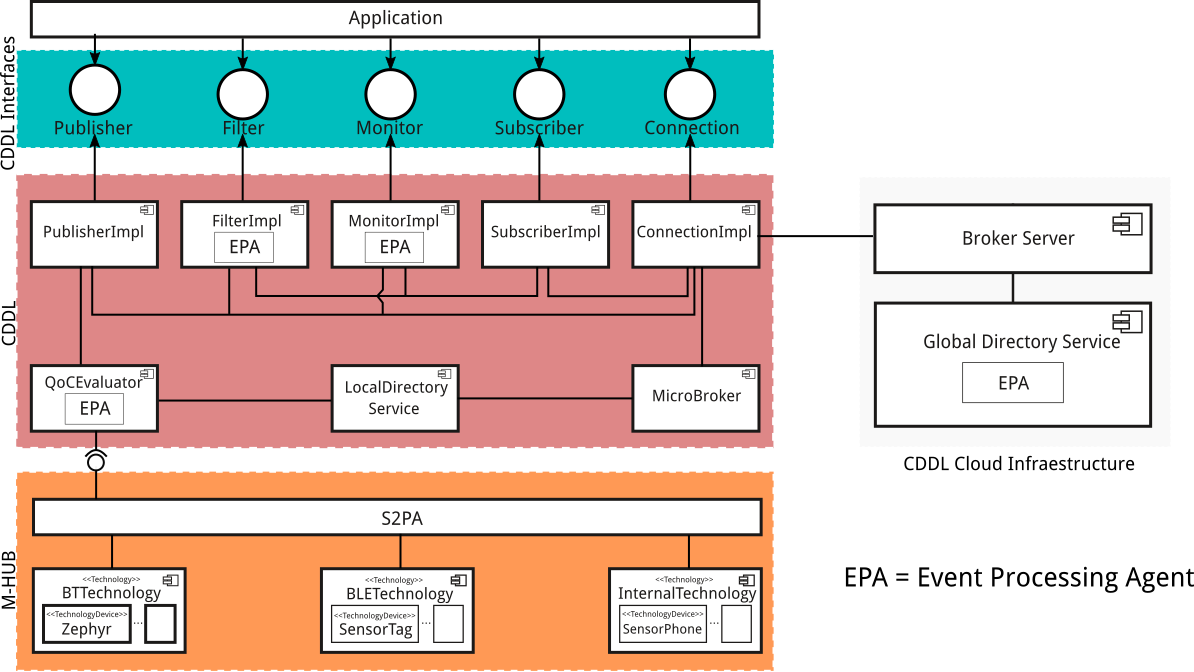
\includegraphics[width=.72\linewidth]{img/mhub-cddl-architecture.png}
		\caption{Fonte: \cite{gomes:et-al:2017}}
	\end{figure}
\end{frame}

\begin{frame}
	\frametitle{\mhub}
	Pode ser definido como um serviço de \middleware de \iomt executado em um dispositivo móvel pessoal, responsável por descobrir e oportunisticamente conectar à \smartobjs acessíveis apenas através de tecnologias WPAN de curto alcance \cite{talavera:et-al:2015}.

	\bigskip
	
	O \smartphone executando o \mhub, funciona como \gateway para \smartobjs, fornecendo acesso à Internet para dispositivos que não podem se conectar.
\end{frame}

\begin{frame}
	\frametitle{\stwopa}
	\begin{itemize}
		\item protocolo que fornece uma \api comum para realizar a comunicação com diferentes tecnologias WPAN;
			
		\item implementado como um módulo na arquitetura do \middleware, define um conjunto de métodos e interfaces que os módulos responsáveis por determinada tecnologia de comunicação devem implementar;
			
		\item fornece uma \api unificada para todas as camadas superiores da arquitetura que precisam se comunicar com tais tecnologias.
			
	\end{itemize}
	
\end{frame}

\begin{frame}
	\frametitle{Interfaces definidas pelo \stwopa}
	\begin{figure}[htb]
		\centering
		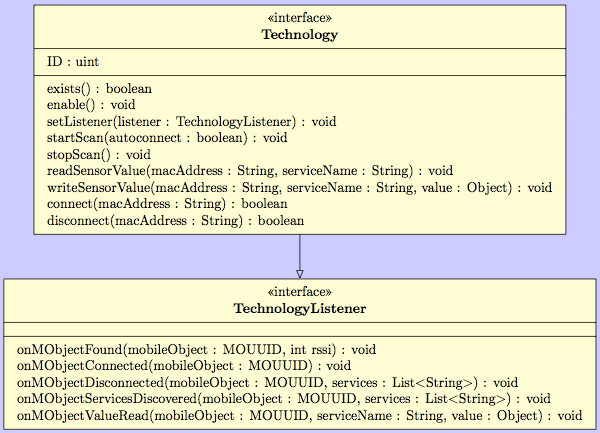
\includegraphics[width=0.55\linewidth]{img/technology-interface.png}
		\caption{Fonte: \cite{talavera:et-al:2015}}
	\end{figure}
\end{frame}

\begin{frame}
	\frametitle{\sensordata}
	Ao receber um evento de descoberta, conexão, desconexão ou leitura de dados, o \stwopa encapula esta informação em um objeto do tipo \sensordata, possuindo os seguintes atributos:
	\begin{itemize}
		\item \texttt{mouuid}

		\item \texttt{signal}

		\item \texttt{sensorName}

		\item \texttt{sensorValue}
			
		\item \texttt{action}
		\begin{itemize}

			\item \texttt{FOUND}

			\item \texttt{CONNECTED}

			\item \texttt{READ}

			\item \texttt{DISCONNECTED}

		\end{itemize}
	\end{itemize}
\end{frame}

\begin{frame}
	\frametitle{\cddl}
	\Middleware \iomt que permite que as aplicações clientes assumam papel de produtoras ou consumidoras de dados de contexto.
	
	\bigskip
	A interação entre produtores e consumidores se dá através do modelo \pubsub com a utilização de \brokers, implementando uma comunicação distribuída com o \mqtt.
	\bigskip
	
	Fornece também um \ubroker que executa internamente no dispositivo móvel.
\end{frame}

\begin{frame}
	\frametitle{A classe \msg}
\end{frame}

\section{Solução proposta}
\section{Referências}

\begin{frame}[allowframebreaks]
	\frametitle{Referências}
	\bibliographystyle{apalike}
	\bibliography{bib/biblio}
\end{frame}

\end{document}
